\section{Ablation Studies}

In ablation studies, we investigated the individual importance of the following modules: curriculum strategy, input and reward normalization, actuator-width information, and the shaped reward. All ablation study experiments were carried with the SAC algorithm with depth perception and one million experience replay buffer size. All training trials took place in the full environment floor scene. We shared the results of ablation studies in the same table as the SAC full environment \ref{table:SACfull}.

Among all ablation variants, only no normalization trial did not provide a working grasp policy. The rest either converged to a lower success rate or converged relatively slower than the baseline. 

Sparse reward and no curriculum learning converged 20 thousand timesteps and 400 thousand timesteps after the baselines. Interestingly, sparse reward SAC agent performed the best in the table scene, on random objects with a 100\% success rate. Both sparse and no curriculum learning trials performed better than the baseline SAC model on wooden blocks in the table scene. Sparse reward and no curriculum learning achieved 72\% and 64\%, while baseline reached 23\%.

No actuator width observation converged to a slightly worse success rate than the baseline.  It achieved a 97\% success rate, while the baseline converged to 99\%. An extra observation related to the environment proved to be useful.

\begin{figure}[htbp]
    \begin{subfigure}{0.49\textwidth}
        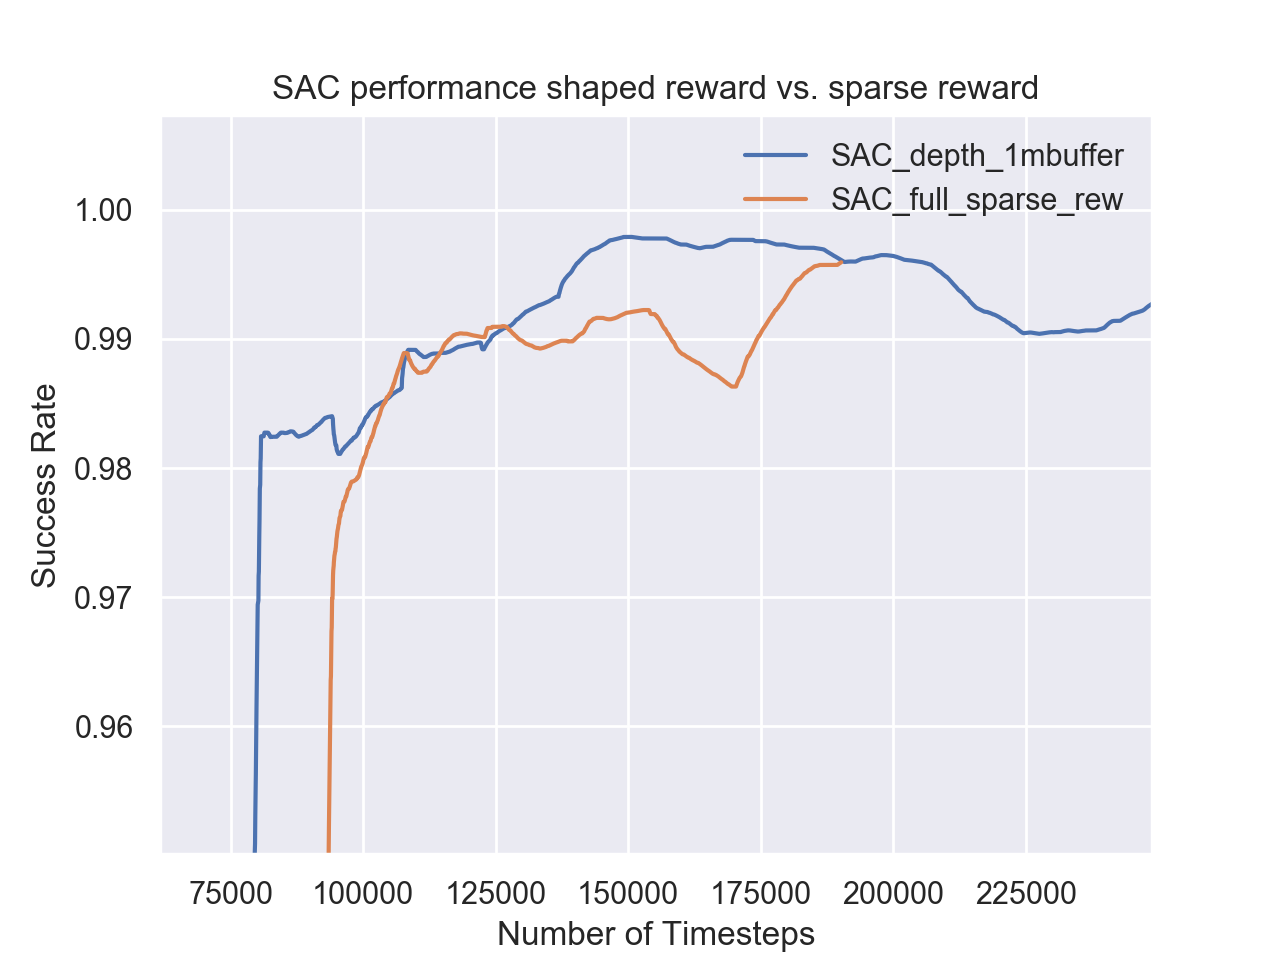
\includegraphics[width=\linewidth]{figures/ablation/SAC_performance_shaped_reward_vs_sparse_reward}
        \caption{SAC performance with shaped reward vs. sparse reward } \label{fig:table}
    \end{subfigure}%
    \hspace*{\fill}   % maximize separation between the subfigures
    \begin{subfigure}{0.49\textwidth}
        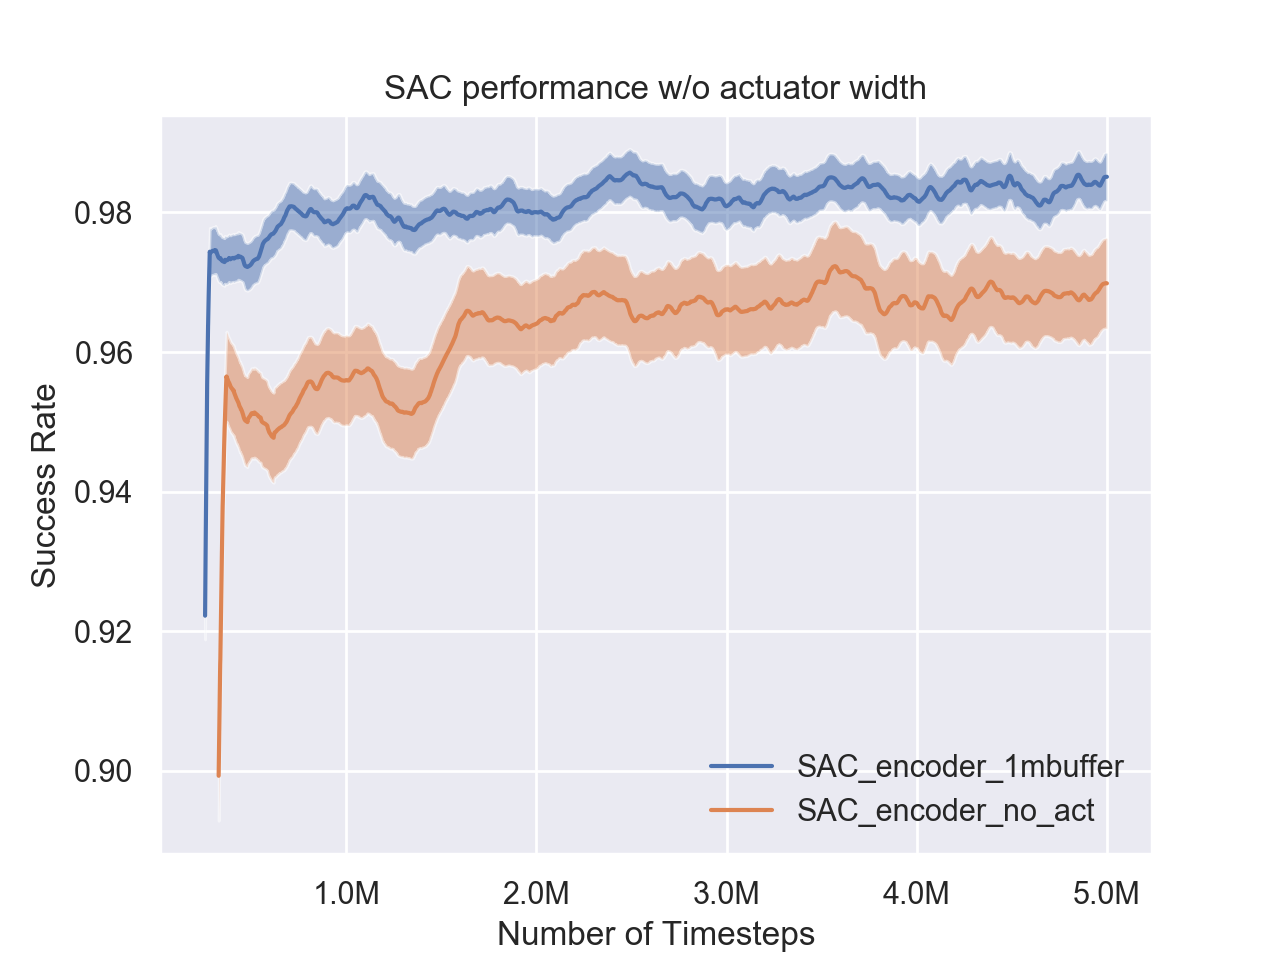
\includegraphics[width=\linewidth]{figures/ablation/SAC_performance_wo_actuator_width}
        \caption{SAC performance with encoder perception without actuator width observation} \label{fig:noact}
    \end{subfigure}%
    \hspace*{\fill}   % maximize separation between the subfigures


\caption{ Ablation of reward function and actuator width observation \label{fig:scenes}}
\end{figure}

\begin{figure}[htbp]
    \begin{subfigure}{0.49\textwidth}
        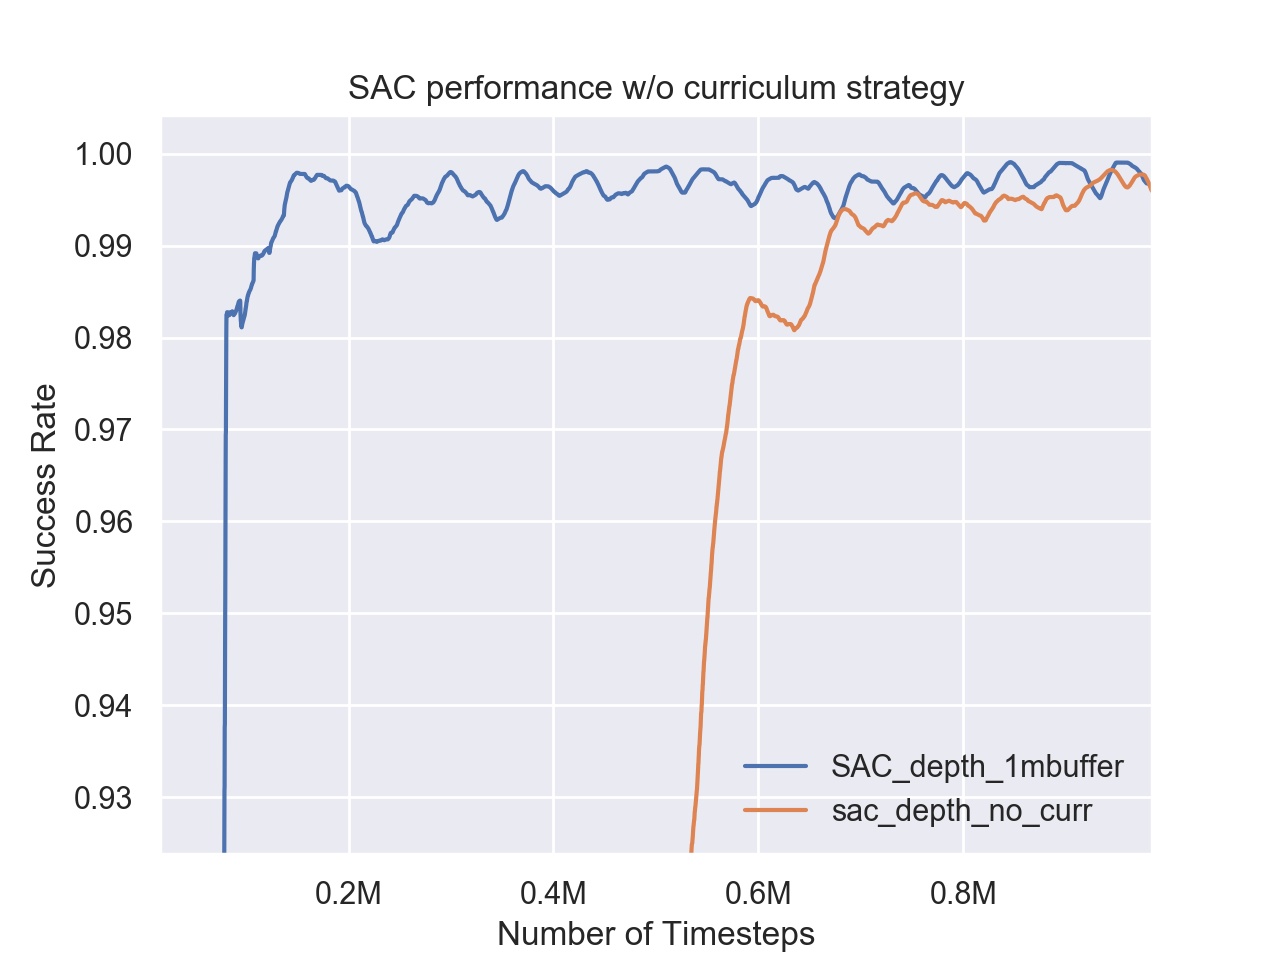
\includegraphics[width=\linewidth]{figures/ablation/SAC_performance_wo_curriculum_strategy}
        \caption{SAC performance withuot curriculum strategy} \label{fig:table}
    \end{subfigure}%
    \hspace*{\fill}   % maximize separation between the subfigures
    \begin{subfigure}{0.49\textwidth}
        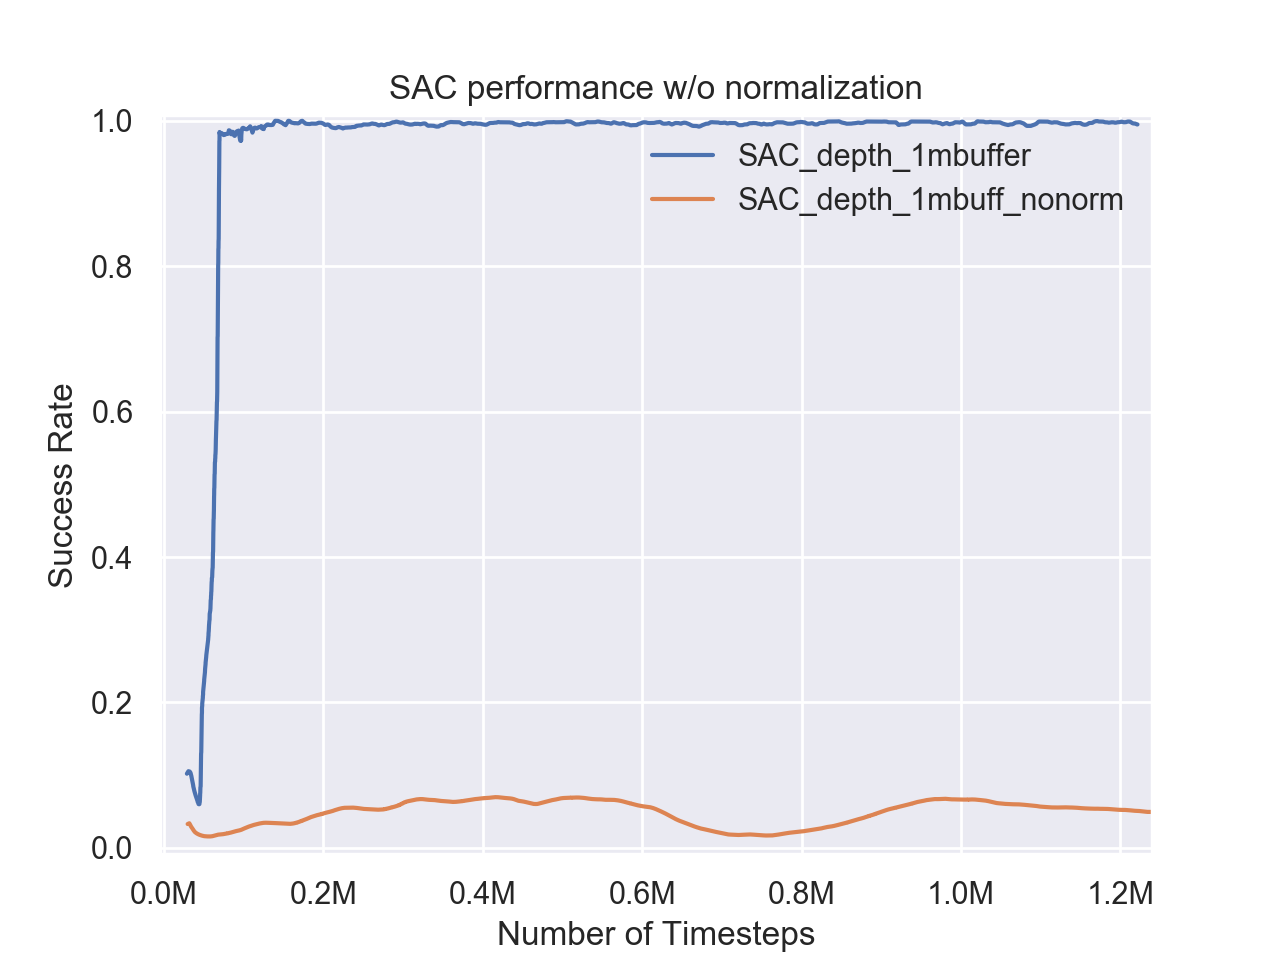
\includegraphics[width=\linewidth]{figures/ablation/SAC_performance_wo_normalization}
        \caption{SAC performance in full environment without normalization compared to the performance of the baseline SAC} \label{fig:nonorm}
    \end{subfigure}%
    \hspace*{\fill}   % maximize separation between the subfigures


\caption{ Ablation of curriculum learning and normalization of input and reward \label{fig:scenes}}
\end{figure}



